\documentclass{article}
\usepackage{geometry}
\usepackage{fancyhdr}
\usepackage{amsmath,amsthm,amssymb}
\usepackage{graphicx}
\usepackage{hyperref}
\usepackage{lipsum}

\usepackage{listings}
\usepackage{xcolor}

\colorlet{punct}{red!60!black}
\definecolor{background}{HTML}{EEEEEE}
\definecolor{delim}{RGB}{20,105,176}
\colorlet{numb}{magenta!60!black}

\lstdefinelanguage{json}{
    basicstyle=\normalfont\ttfamily,
    numbers=left,
    numberstyle=\scriptsize,
    stepnumber=1,
    numbersep=8pt,
    showstringspaces=false,
    breaklines=true,
    frame=lines,
    backgroundcolor=\color{background},
    literate=
     *{0}{{{\color{numb}0}}}{1}
      {1}{{{\color{numb}1}}}{1}
      {2}{{{\color{numb}2}}}{1}
      {3}{{{\color{numb}3}}}{1}
      {4}{{{\color{numb}4}}}{1}
      {5}{{{\color{numb}5}}}{1}
      {6}{{{\color{numb}6}}}{1}
      {7}{{{\color{numb}7}}}{1}
      {8}{{{\color{numb}8}}}{1}
      {9}{{{\color{numb}9}}}{1}
      {:}{{{\color{punct}{:}}}}{1}
      {,}{{{\color{punct}{,}}}}{1}
      {\{}{{{\color{delim}{\{}}}}{1}
      {\}}{{{\color{delim}{\}}}}}{1}
      {[}{{{\color{delim}{[}}}}{1}
      {]}{{{\color{delim}{]}}}}{1},
}



\title{PoET: A Power Efficient, Scalable Consensus Algorithm }
\author{Mic Bowman \\ \url{mic.bowman@intel.com}}
\date{2016-Jun-15}
\begin{document}
\maketitle
%\tableofcontents
%\newpage

%% -*- fill-column: 120; -*-
\section{Introduction}
\label{sec_introduction}

Over the last several years, cryptographic currencies like Bitcoin~\cite{} started a disruption that has grown
well-beyond currency. Inspired by the decentralization of fiduciary authority represented by Bitcoin, businesses and
governments across the world are investigating disintermediated and decentralized services. Usages are diverse:
federated identity, clearing and settlement of financial transactions, multi-party supply chain management, provenance
of food, and privacy-preserving access to medical records. At the core of this revolution is a data structure called a
{\it blockchain}. Simply put, a blockchain is a data structure that uses cryptographic hashes to create an immutable
ordering of events. Communities use blockchains to represent a shared view of ``truth''. For example, when events like
``transfer \$50 from john to jane'' or ``grant tom access to file A'' are committed to a blockchain, the entire
community agrees that the event occurred and can act accordingly.

There are many ways for a community to build and maintain a blockchain. In some cases, a trusted organization (like a
representative consortium or a contracted infrastructure provider) can build a blockchain using fairly traditional
distributed database technologies. However, for those cases where no trusted organization exists building a blockchain
requires a protocol that creates consensus across the community about the current, correct state of the blockchain.
There are many different protocols for building consensus based on requirements related to performance, scalability,
consistency, threat model, and failure model. Traditionally, protocols that achieve consensus for arbitrary
(i.e. Byzantine) faults require several rounds of explicit voting. While this approach provides high throughput and
finality of commits, its reliance on a well-known, generally static voting block and the heavy use of communication
(multiple rounds of $N^2$ messages) limit its use to reletively small, localized, and stable applications. 

Bitcoin introduced a new method for achieving consensus, called Nakamoto consensus, that supports broad participation
from a dynamic group of participants. Nakamoto consensus relies on uncoordinated, distributed leader election that is
efficient for communication, but often very computationally intense. For example, Bitcoin elects the leader using
``proof-of-work'', a race to solve a cryptographic puzzle through repetitive ``guess and test''. The first participant
to solve the puzzle is granted unilateral authority to propose the next block that will be added to the blockchain.
While Nakamoto consensus provides a global agreement protocol that is highly resilient to faults, the computational
characteristics of proof-of-work drive processing to custom hardware that can consume gigawatts of power~\cite{}.

This paper describes a new leader election algorithm designed for Nakamoto consensus, called ``Proof of Elapsed Time''
or PoET, that elects leaders through a simple computation in a trusted execution environment provided by commodity
processors.  PoET is based on the observation that proof-of-work, at its core, is a method for generating and enforcing
random wait times--proof-of-work elects as leader the first participant to solve the cryptographic puzzle, a time that
is a random interval drawn from an exponential distribution. With PoET, participants use Intel's Software Guard
Extensions (SGX)~\cite{} to generate and then enforce a random wait time without the cryptographic puzzle. Where
proof-of-work can verify correctness by providing the solution to the puzzle, PoET uses an attestation of correctness
that is provided by the trusted execution environment; any participant can verify that the wait time was generated
correctly and enforced.  In this way PoET preserves the fairness and integrity of leader election provided by
proof-of-work without high cost of electricity and custom hardware. This allows deployment of highly-resilient, fault
tolerant applications for a dynamic community using commonly available computing resources.

% -----------------------------------------------------------------
%% Unfortunately, there are a variety of limitations that handicap the block chain in its current
%% instantiation and prevent it from being used for other (potentially) useful purposes. We focus on
%% leveraging Intel's SGX environment [AGJS13] to re-engineer the proof of work to a proof of wait,
%% creating a new lottery-based consensus protocol. This will provide greater efficiency and reduce
%% the amount of energy used and high costs that we currently see.

%% The key concept of the proof of wait is a guaranteed wait time, provided through the Trusted
%% Execution Environment (TEE) that we get with SGX. Each \miner" will request a wait time from
%% the TEE, and the miner with the lowest wait time \wins," thus getting to create the next block.
%% In order to prove that the node did indeed wait the claimed time, an attestation is also created
%% within the TEE. This validation will be done using the Enhanced Privacy ID (EPID) [BL07, BL09]
%% scheme

For the purpose of achieving distributed consensus efficiently, a good leader election function has several
characteristics:

\begin{itemize}
\item Fairness:
  The function should distribute leader election across the broadest possible population of participants.

\item Investment:
  The cost of controlling the leader election process should be proportional to the value gained from it. 

\item Verification:
  It should be relatively simple for all participants to verify that the leader was legitimately selected. 
\end{itemize}

The PoET leader election algorithm meets the criteria for a good lottery algorithm. It randomly distributes leadership
election across the entire population of validators with distribution that is similar to what is provided by other
lottery algorithms. The probability of election is proportional to the resources contributed (in this case, resources
are general purpose processors with a trusted execution environment). An attestation of execution provides information
for verifying that the certificate was created within the TEE (and that the validator waited the allotted
time). Further, the low cost of participation increases the likelihood that the population of validators will be large,
increasing the robustness of the consensus algorithm.

% goal open population of validators
% threat model

%% -*- fill-column: 120; -*-
\section{Distributed Consensus}
\label{sec_priorart}

% -----------------------------------------------------------------
% -----------------------------------------------------------------
\subsection{Byzantine Fault Tolerance}

Describe Byzantine Generals problem.

Describe PBFT family of algorithms

The Good:
\begin{itemize}
\item Performant
\item Finality
\end{itemize}

The Challenges:
\begin{itemize}
\item Lots of communication
\item Sensitive to network conditions
\item Identity of all participants must be known
\end{itemize}

Limited decentralization.

% -----------------------------------------------------------------
% -----------------------------------------------------------------
\subsection{Nakamoto Consensus}

Describe Nakamoto Consensus as implemented in Bitcoin.

Replace finality with eventual consistency (probabalistic)

Proof of work as leader election and sybil prevention.

Implicit voting.

The Good:
\begin{itemize}
\item Decentralization of authority and implementation
\end{itemize}

The Challenges:
\begin{itemize}
\item Proof of work is extremely expensive
\end{itemize}

Properties of leader election in Nakamoto Consensus
\begin{itemize}
\item Uses distribution in time to optimize communication. A good leader
  election algorithm distributes election over time to increase the
  probability that only one broadcast is necessary.
\item Resistant to censorship
\item Adapts to population changes
\end{itemize}

% -----------------------------------------------------------------
% -----------------------------------------------------------------
\subsection{Trusted Execution}


%% -*- fill-column: 120; -*-
\section{PoET: Proof of Elapsed Time}
\label{sec_poet}


At the beginning of each consensus round, a validator builds a block that extends the chain it believes to be the
correct one (note that the selection of a chain to extend is an implicit ``vote'' for the chain). Next, the validator
performs a computation that determines a time duration it must wait before it may claim leadership and extend the chain
with the block it constructed. If no one claims leadership before the time expires, the validator broadcasts
its proposed block and a proof that it computed the time correctly. The chain is extended with the new block and the
process begins again. 

The future time that is computed represents a form of ``lottery'' where every validator is given a ticket and the
validator with the smallest ticket wins the lottery. The computation used to generate the lottery ticket must meet
several important criteria:

To provide resiliency to Byzantine faults:
\begin{itemize}
\item Censorship Resistant
  The computation should distribute leader election across the broadest possible population of participants. Fairness
  ensures that no single validator can persistently control the transactions that may be committed; that is, fairness
  ensures censorship resistence.

\item Sybil Prevention
  The cost of controlling the leader election process should be proportional to the value gained from it. Investment
  limits the potential for an organization to control consensus by ``flooding'' the process with voters without a
  corresponding investment of resources. Investment democratizes consensus. 
\end{itemize}

To ensure efficient execution:
\begin{itemize}
\item Distribute Wait Times
  The communicatio nefficiency of Nakamoto consensus is a result of implicit voting and 

\item Simplify Verification
  While the cost of computing the lottery function should be high to ensure investment, it should be relatively simple
  for all participants to verify that the function was performed correctly. This asymetry in computation ensures that
  false leadership claims can be identified quickly and rejected.

\item Adapt to Changing Populations

\end{itemize}




Nakamoto consensus involves an uncoordinated, distributed leader election.

Leader election must be easily verifiable.
This is efficient if the leader can be established with a single broadcast. 

Nakamoto consensus is efficient when all validators accept a leader with a single broadcast.
Distributed in time such that a single node believes it is at the front of the line and has time to communicate that
fact to all other nodes before any other node believes it is at the front of the line.

\begin{center}
  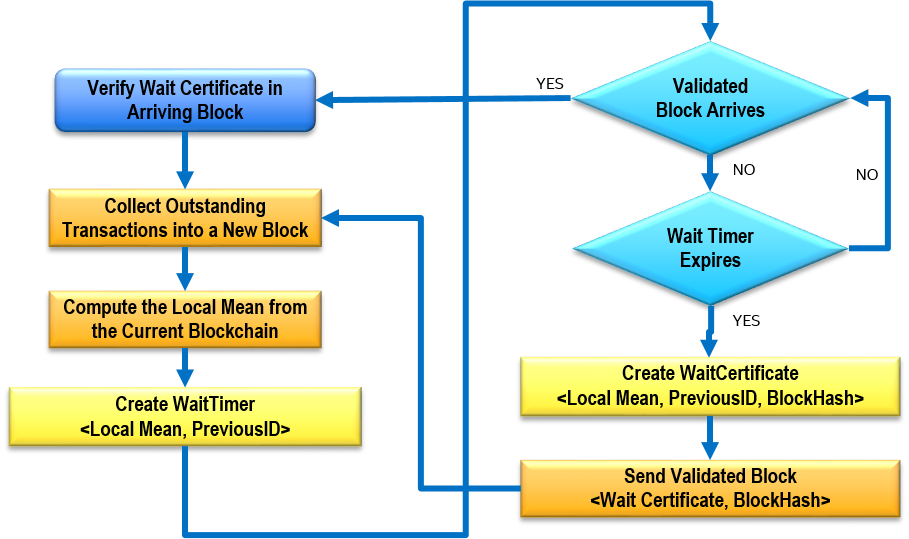
\includegraphics[scale=.75]{figures/PoET_Flow.png} \
  \caption{Control flow in the PoET protocol}
  \label{fig:poetflow}
\end{center}

\subsection{Local Mean Computation}

\subsection{Fork Resolution}


% basic poet algorithm indenpdent of the enclave
% initialization/slow start
% flow control: create timer, when timer expires, create cert, verify cert
% configuration parameters
% population dynamics with computation of local mean
% handling forks, single block selection, multiple block
% chains... largest aggregate local mean, rationale for why this works
% evaluation of local mean adaptation

%% -*- fill-column: 120; -*-
\section{Building the Enclave}
\label{sec_enclave}

In this section we describe how the PoET enclave is used to implement the election protocol of our blockchain.  The
protocol consists of two phases: \textit{the sign-up} phase and the \textit{election} phase.


% high level description of the enclave interface
% signup phase, create wt, create wc, verify wc
% enclave evaluation... various attacks and the solutions

% Naive approach to validation results in horrible performance. Added
% signup phase to offload validation, implications for revocation

% dependence on ME for time; the threat for attacks. Not really a
% problem since the tie breaker ensures correctness and progress. But
% important for DOS prevention

% wait cert bound to a block --> blockhash, why we can do late binding
% by adding allowing one wait cert per wait timer (only get one chance,
% can't game wait cert creation by trying different blockhashes)
% wait cert bound to a validator --> validator public id in the blockhash
% multiple instances of an enclave --> monotonic counter in the signup info
% multiple signup attack --> validation policy requires N blocks before
% registration complete
% recourse: revocation....

Multiple instances of the enclave
Problem: Multiple instances of an enclave implies multiple votes
Solution: Bind the ID of a monotonic counter to the EPID pseudonym
during sign up 

Restarting the enclave repeatedly to get a better identity
Problem: Signature of the WC is used in the wait time computation
implies PSK/PPK pair can influence the wait time point of control 
Solution: Ledger implements policy to force multiple blocks to commit
before an identity ledger randomness prevents meaningful control

Late binding of transactions improves performance, but provides control point
Problem: Block hash is used in wait time computation implies TXN list can influence future wait time
Solution: At most one WC may be created for a WT

Wait Certificate can be lifted and placed in a different block
Problem: Separation of ledger and enclave identities allows WC to be lifted from the block
Solution: Bind WC to persistent ledger identity, not just enclave identity

%% -*- fill-column: 120; -*-
\section{Circuit Breaker}
\label{sec_failure}

As you know, we cannot stop a validator with a compromised enclave from
winning a validation round. A compromised enclave can create a bogus
wait certificate with a very short duration that would ensure that it
wins a given round. Our goal with respect to compromised enclaves is to:

\begin{enumerate}
\item Make it as hard as possible to compromise the enclave
\item Ensure that a compromised enclave cannot compromise the
  correctness of the ledger
\item Ensure that the ledger can continue to progress (that is, correct
  valiators will continue to accept, validate and commit new
  transactions) in spite of a ``reasonable'' number of compromised enclaves
  (assume at most 1/3 compromised validators).
\end{enumerate}

Andrea's work addresses the first goal. The separation of
consensus and correctness testing addresses the second goal. That leaves
the third goal to be addressed.

We have proposed some form of limitation on the frequency with which a
given validator can win lotteries as a means to address the third
goal. Limiting the frequency of wins (with the assumption that a
reasonable number of validators are correct) ensures that correct
validators will be able to commit a significant proportion of the
blocks. That is, compromised nodes might be able to degrade performance
of the ledger by committing correct, but potentially "meaningless",
blocks, but compromised nodes cannot prevent progress by correct
validators.

Originally we described the method of limiting frequency as an "M of N"
policy. That is, a given validator could win at most M lotteries out of
N blocks. That policy would work for a more or less consistent pool of
validators. However, the population of validators constantly
changes. And the values of M and N depend heavily on the population
size.

As an alternative I'm proposing that we use a "1 sample z test" (see [1]
and [2] below for more information). A "1 sample z test" computes the
value of the standard deviation of a specific observation relative to
the expected value. So the z value computed for a set of observations is
the number of standard deviations the observations are from the
expectation. To be concrete, with a population of 1000 validators, the
probability of winning is 1/1000. That means that for a sample of 100000
blocks, a validator would be expected to claim 100 blocks. If we observe
that a validator has actually won 125 blocks, that would mean the z
value would be about 2.5. We can then use the z value to compute the
probability that a given validator is winning more often than it
should. For example, with 99.5\% confidence, we can say that The "1
sample z test" has many nice properties: It allows for variance in
winning. It is not constrained to a specific time period so it can apply
to both recent performance and historic performance. A correct validator
can apply the test before it claims a block to know if claiming the
block would put outside of acceptable behavior (which means we can
remove "false positives" where the algorithm would falsely determine
that a correct validator is behaving incorrectly).

I have run a number of simulations with 100000 blocks over a dynamic
population of validators with a mean of around 1000. When I run the "1
sample z test" with a correct validator and a 99.5\% confidence interval
(the validator should win about 1 block out of 1000), I get a false
positive in about 5\% of the runs. A validator winning at a rate of 2
blocks out of 1000 was caught in every run, generally within a few
hundred blocks. To be clear, the test means that we check the statistic
for every prefix of the chain (did the validator win too often in the
last 10 blocks? The last 11 blocks? The last N blocks?). That way we
can identify bad behavior at any scale.

There are several ways to configure the algorithm: 

\begin{itemize}
\item The number of observations required before any test is considered
  valid (a validator must win at least 3 blocks before the test is
  applied by default)

\item The amount of "history" we consider (the default is to examine the
  entire chain)

\item The confidence interval (the default is 95\% though I have found
  that for large validator pools, 99.5\% provides very good numbers)

\item The "initialization" period (how many blocks have to be committed
  before we start testing)
\end{itemize}

That last parameter makes testing a big pain. Since the initialization
of the ledger does not use the probabilistic sampling to get wait times,
it has completely bogus numbers for the population of validators. So
there need to be enough blocks in the ledger to make the sampling an
accurate representation of the number of validators. I'm still playing
with that number; trying to see if there is any other way handle start
up more rationally.

The implementation uses a cache of population estimates that is
maintained by the journal layer (PoetJournal). The cache is a dictionary
that maps a block id to the identity of the validator of the block, the
population estimate from the WaitCertificate and the previous block
identifier. When a validator claims a block, the test computes the z
value for that validator for every prefix of the chain (rooted at the
current block). I'm fairly certain there are more efficient ways to do
the computation (how far do we have to look back through history to
determine that this one last block pushed the z value over the
threshold). Though even for 100000 blocks the time to compute isn't too
bad (< 1 second).

I have two concerns with the algorithm:
\begin{itemize}
\item There is a potential for a feedback loop. Taken to the extreme,
  this algorithm would result in round robin behavior (which is not
  necessarily a bad thing). If a validator wins a lottery, it might take
  itself out of the population while it waits for its next turn. That
  has an effect on the population estimates. Lower population estimates
  allow for validators to win more often. So the validator re-joins when
  it would be allowed to win. I think the system would stabilize but I
  don't know what the characteristic would be (e.g. for 1000 actual
  validators that are all playing by the rules, the population estimates
  might actually be closer to 500).

\item Bad things could happen if the validator population changes very
  quickly. For example, say that we start with 1000 nodes and the
  network is partitioned with 500 in each half. Could we end up in a
  situation where *NO* node could win the next lottery? I've seen
  something like this in the initialization where the population
  estimate is much larger than the actual population. If enough blocks
  are committed then the population estimate adjusts enough to
  accommodate. However, blocks have to be committed before the
  adjustment can be made.
\end{itemize}

Reproducing both of these situations is nearly impossible with an actual
ledger. I need to build a more robust simulator to convince myself that
bad things won't happen.

%[1] http://www.cogsci.ucsd.edu/classes/SP07/COGS14/NOTES/binomial_ztest.pdf
%[2] http://www.statisticslectures.com/topics/onesamplezproportions/


%% -*- fill-column: 120; -*-
\section{Evaluation}
\label{sec_evaluation}

This is the evaluation section.

% experimental evaluation
% did it work... number of forks, resolution of forks
% local mean adaptation
% performance impact of compromised enclaves and overclocked timers

%% -*- fill-column: 120; -*-
\section{Summary}
\label{sec_summary}

This is the summary section.


\begin{thebibliography}{9}
\end{thebibliography}
\end{document}
